% (C) Marc Lijour, 2019 
% Licensed under a Creative Commons License BY-SA
% https://creativecommons.org/licenses/by-sa/2.5/ca/
% Presentation for the Blockchain Developer Certificate students at George Brown College
% ICOs and elements of a white paper

\frame{ 
	\frametitle{ICOs --the good, the bad, and the ugly}
    \begin{block}{About the Genesis of Blockchain networks}
    Bitcoin started the Blockchain phenomenon as a peer-to-peer network, which compensates peers for running its software on their own computers.\\
    What do you do with Bitcoins?
    \end{block}
}

% ======================================================================================================
%                         What are ICOs? 
% ======================================================================================================
% - context, definition
% - process
% - examples (pointing a view, no details)
\section{What are ICOs?}

\subsection{Definitions}
\frame{ 
	\frametitle{A definition of Initial Coin Offering (ICO)}
    \begin{block}{Mirriam Webster}
    an initial offering of a cryptocurrency to the public
    \end{block}

    \emph{\small Also called ITO, for Initial Token Offering.}
}

\frame{
% 
	\frametitle{Distinction: Cryptocurrency vs. ICOs}
	\begin{figure}
		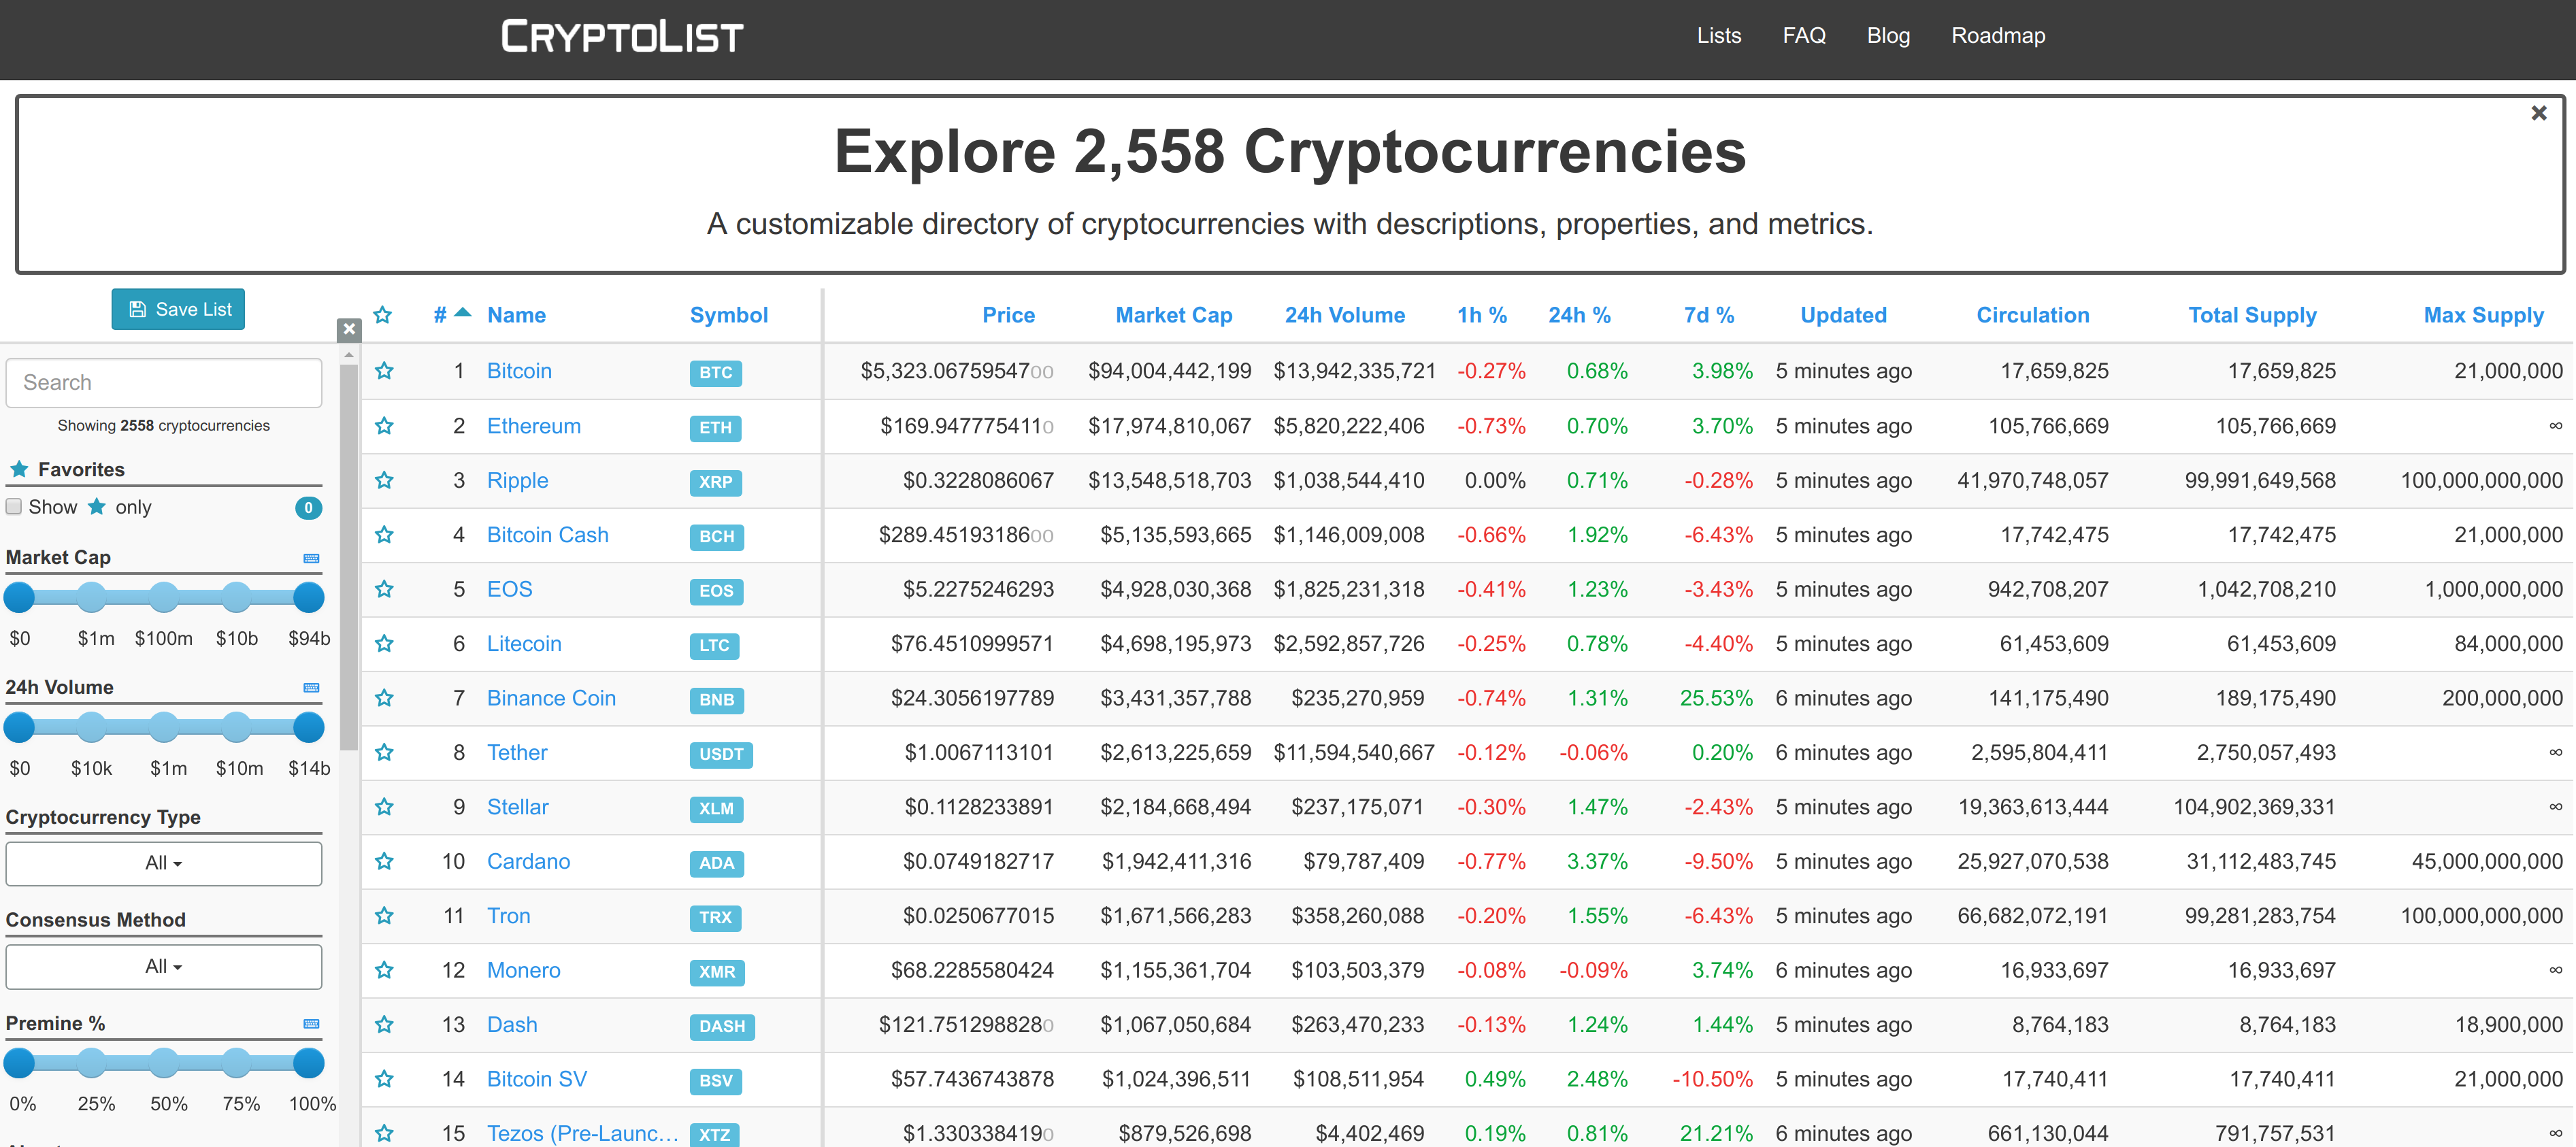
\includegraphics[width=10.5cm]{../pics/cryptocurrency/cryptolist-en}
	\end{figure}
}

\frame{ 
	\frametitle{Distinction: Cryptocurrency vs. ICOs}
    \begin{alertblock}{Cryptocurrency (Oxford dictionnary)}
     a digital currency in which encryption techniques are used to regulate the generation of units of currency and verify the transfer of funds, operating independently of a central bank.
    \end{alertblock}

    \begin{exampleblock}{ICO}
     a fundraising mechanism leveraging the issuance of a cryptocurrency.
    \end{exampleblock}
}

\frame{
% https://medium.com/theventurecity/who-finances-the-startup-journey-96be3a9fccae
	\frametitle{Source of funding for startups}
	\begin{figure}
		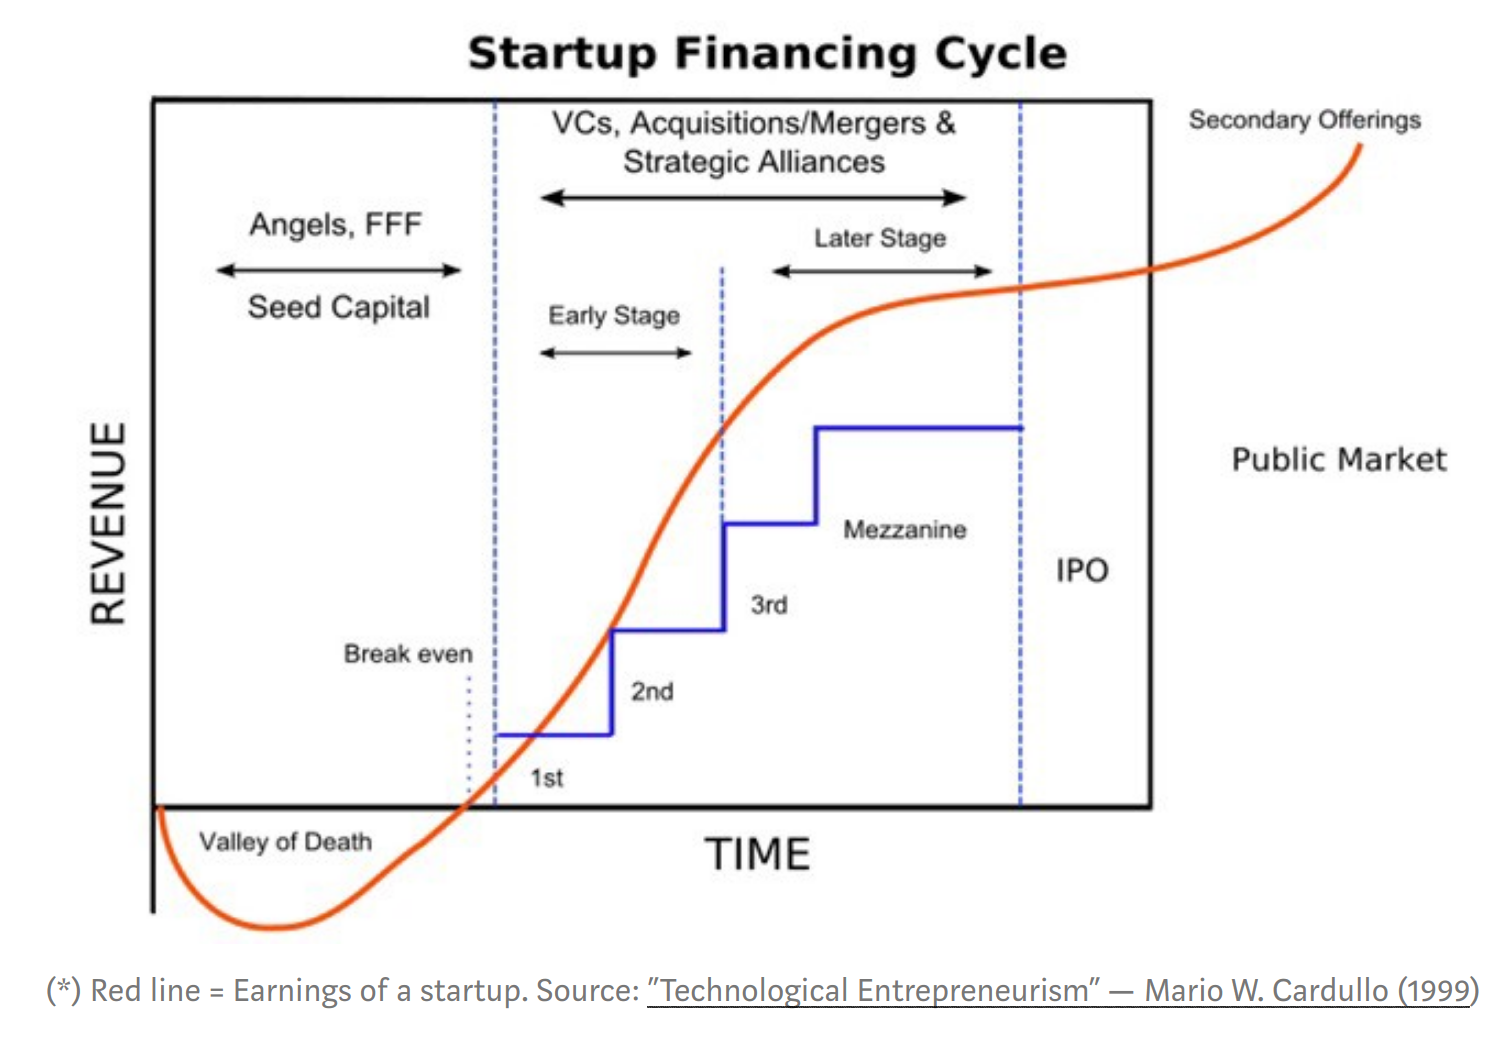
\includegraphics[width=10.5cm]{../pics/startups/startup-financing-cycle}
	\end{figure}
}

\frame{ 
	\frametitle{IPO vs. ICO}
	\begin{columns}
	\column{0.5\textwidth}
    \textbf{IPOs}
    \begin{itemize}
        \item need a prospectus
        \item need an underwriter (big bank e.g. JP Morgan)
        \item sales on exchanges
        \item regulatory constraints
    \end{itemize}
	\column{0.5\textwidth}
    \textbf{ICOs}
    \begin{itemize}
        \item white paper
        \item anyone can launch a sale
        \item anyone can buy from anyone
        \item no limitation allowing schemes such as "pump and dump"
    \end{itemize}
    \end{columns}
}

\frame{
    \frametitle{IEO vs. ICO}
	\begin{columns}
	\column{0.5\textwidth}
    \textbf{Initial Exchange Offering (IEO)}
    \begin{itemize}
        \item register with an exchange
        \item pay a fee and a \% of coins
        \item sales happen on the exchange
        \item regulatory burden for the exchange
        \item marketing and promotion on the exchange
    \end{itemize}
	\column{0.5\textwidth}
    \textbf{ICO}
    \begin{itemize}
        \item true peer to peer
        \item no fees to intermediaries
        \item anyone can buy from anyone
        \item regulatory burden on the promoters of the ICO
        \item developers have to promote themselves
    \end{itemize}
    \end{columns}
    \vspace{1em}
    {\small    
        See \url{https://cryptonews.com/guides/what-is-an-initial-exchange-offering.htm}
    }
}

\frame{
    \frametitle{Who buys into ICOs?}

    \center\Huge  Discussion
}

\frame{ 
% https://cointelegraph.com/news/new-study-says-80-percent-of-icos-conducted-in-2017-were-scams
	\frametitle{Notable ICO scams}
    \begin{itemize}
        \item the team runs with the investor's money (e.g. Modern Tech’s Pincoin ICO)
        \item misrepresentation of the team (e.g. fake founders in the case of Benebit)
        \item Ponzi schemes (e.g. Ponzicoin --it's in the name!; Plexcoin promised a 1,354\% return to US and Canadian investors)
        \item market manipulation (e.g. "pump and dump")
        \item marketing schemes (e.g. Kodack coin, Centratech ICO backed by DJ Khaled)
    \end{itemize}
}

\frame{ 
    \frametitle{And the laws says\ldots}
    \begin{block}{SEC (US Regulator)}
% TODO add to bib
    \href{https://www.sec.gov/files/dlt-framework.pdf}{Framework for “Investment Contract” Analysis of Digital Assets} (2019)
    \end{block}

    \begin{block}{OSC (Ontario Regulator)}
    \href{https://www.getsmarteraboutmoney.ca/invest/investment-products/cryptoassets/}{OSC Investor Guide to Crypto Assets} (2019)
    \end{block}
}

\frame{
    \frametitle{A few instruments and tools}
    In 2017, the SEC provided guidance on the sale of token, indicating that it would be (most likely) treated as a security.

    \begin{block}{The Howey test}
    Simply put: if it looks like an investment, then it is one. \\
    \emph{\small The Howey Test refers to a 1946 case which reached the Supreme Court, SEC v. W.J. Howey Co., involving the Howey Company of Florida.}
    \end{block}

    \begin{alertblock}{Investment contracts}
    A promise to return a profit on an invesment.
    \end{alertblock}
}

\frame{
    \frametitle{A few instruments and tools}
    \begin{block}{SAFT}
    A Simple Agreement for Future Tokens (SAFT) is an assumed investment contract (a security) that brings clarity to the sale of Blockchain-based securities. \\
    \vspace{0.5em}
    \emph{User receives documentation and access to the future token sale. It's not a debt instrument.}
    \end{block}

    \begin{block}{SAFE}
    A Simple Agreement for Future Equity (SAFE) allows to accept funds that can be converted to equity at a later stage.
    \end{block}
}

\frame{ 
	\frametitle{Finding the right balance}
	\framesubtitle{Let's discuss}
    \begin{block}{Democratization of access to capital}
    What is the best way to let small investors access lucrative investment opportunities generally available to accredited investors and large portfolio owners?
    \end{block}

    \begin{exampleblock}{Support for innovation}
    What is the best way to allow startups to access the capital they need at a reasonable cost?
    \end{exampleblock}

    \begin{alertblock}{Protection of the investors}
    What is the best way to protect investors against evil market manipulations? (Let's discuss some of those)
    \end{alertblock}

}

\frame{ 
	\frametitle{Other approaches to coin offerings}
    \begin{itemize}
        \item Initial Bounty Offering
        \item Security Token Offering (more details later)
        \item Initial Exchange offering
        \item \ldots
    \end{itemize}
}

% ---------------------------------------------------
\subsection{Market size}

\frame{
    \frametitle{}

    \center\Huge  Market Size
}

\frame{
% 
	\frametitle{Top 10 ICOs}
	\begin{figure}
		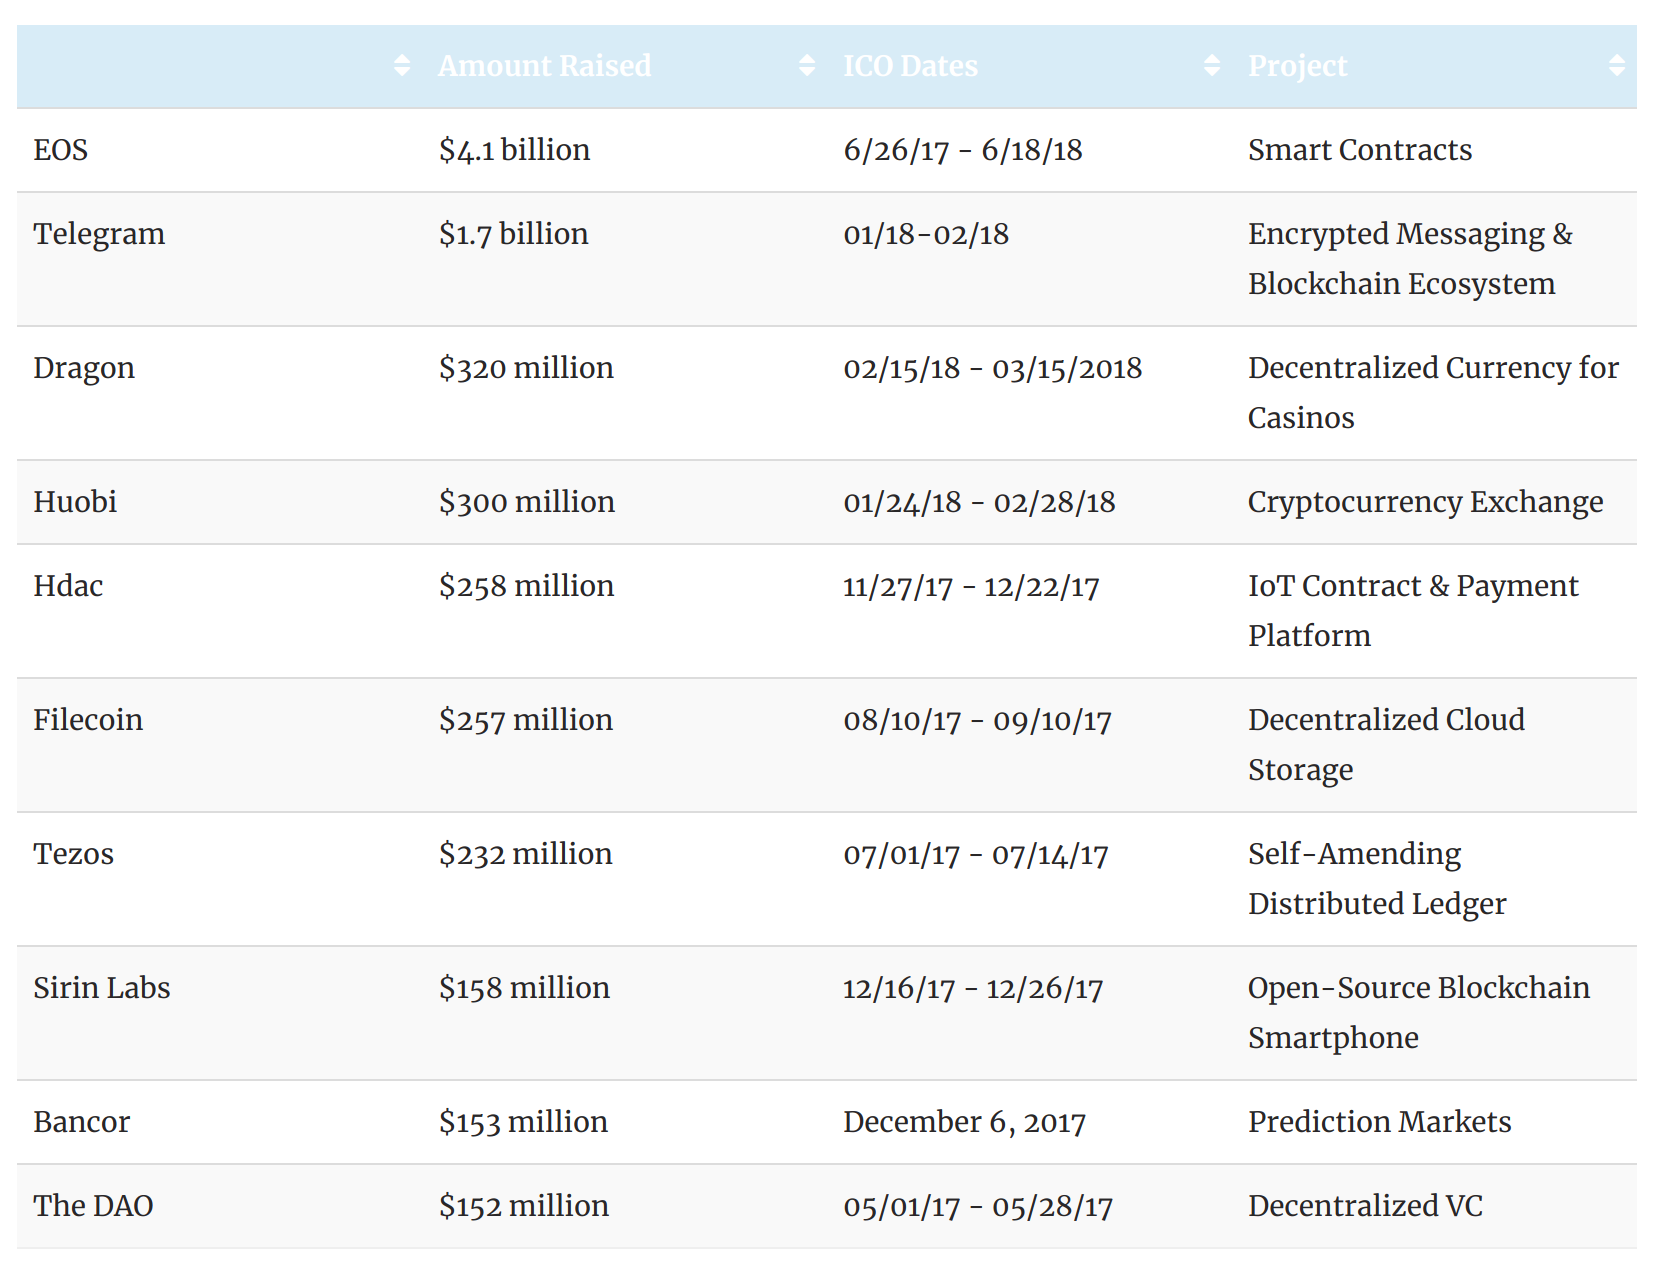
\includegraphics[width=10.5cm]{../pics/cryptocurrency/top10-icos-2018-short}
	\end{figure}

    See also the ICO rektness 2014--2018 table compiled by Alyze Sam.
    \url{https://docs.google.com/spreadsheets/d/19UbHf6PwVqivyCzVkiPmaTvk23Ig5YHwFWLwSyu8ffQ/edit\#gid=1772156349}
}



\frame{
% https://www.investinblockchain.com/invest-in-icos/
	\frametitle{Proportion of funds raised through ICOs}
	\begin{figure}
		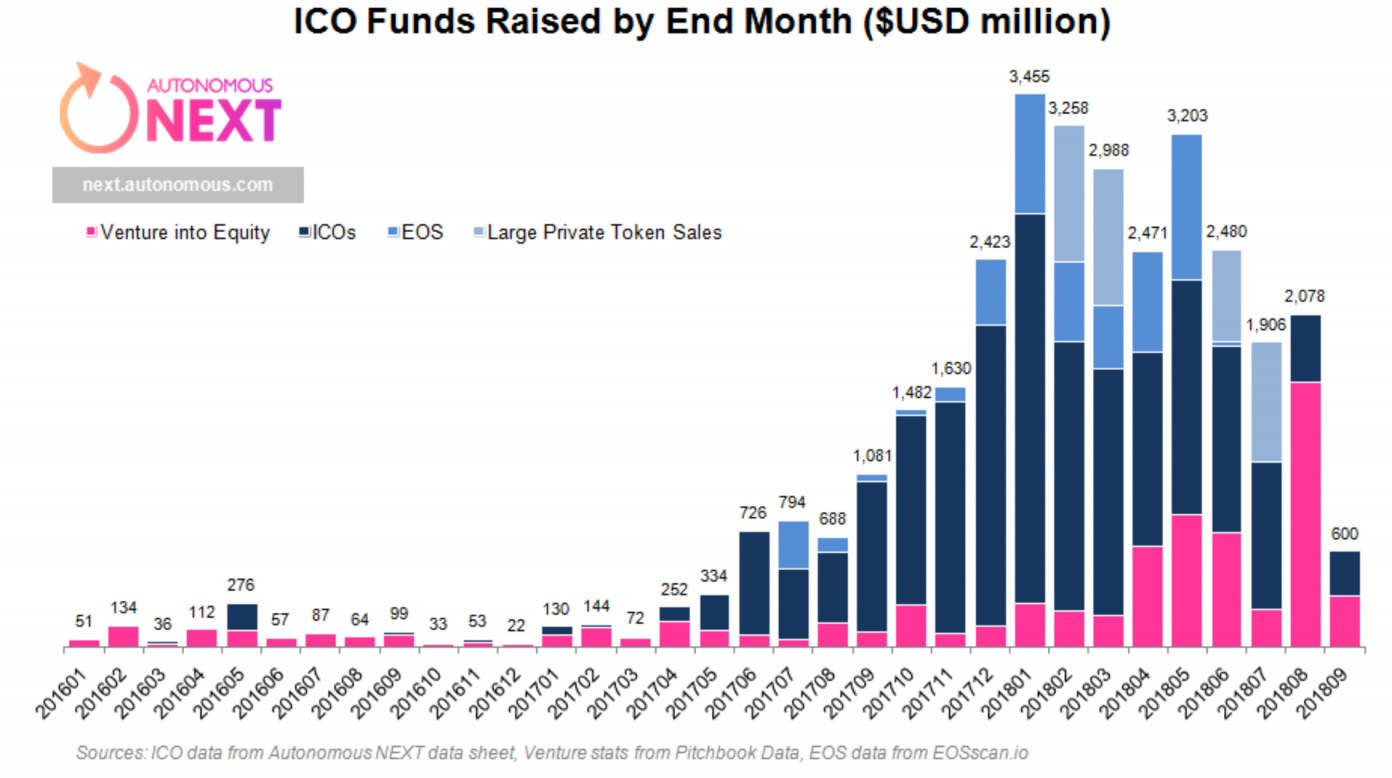
\includegraphics[width=10.5cm]{../pics/cryptocurrency/2016-2018-autonomous-research-ico-funds-raised}
	\end{figure}
}


\frame{
% https://www.linkedin.com/posts/vladyslavskakun_cryptodiffer-on-twitter-activity-6598988003492798464-GI7f
	\frametitle{Proportion of funds raised through IEOs}
	\begin{figure}
		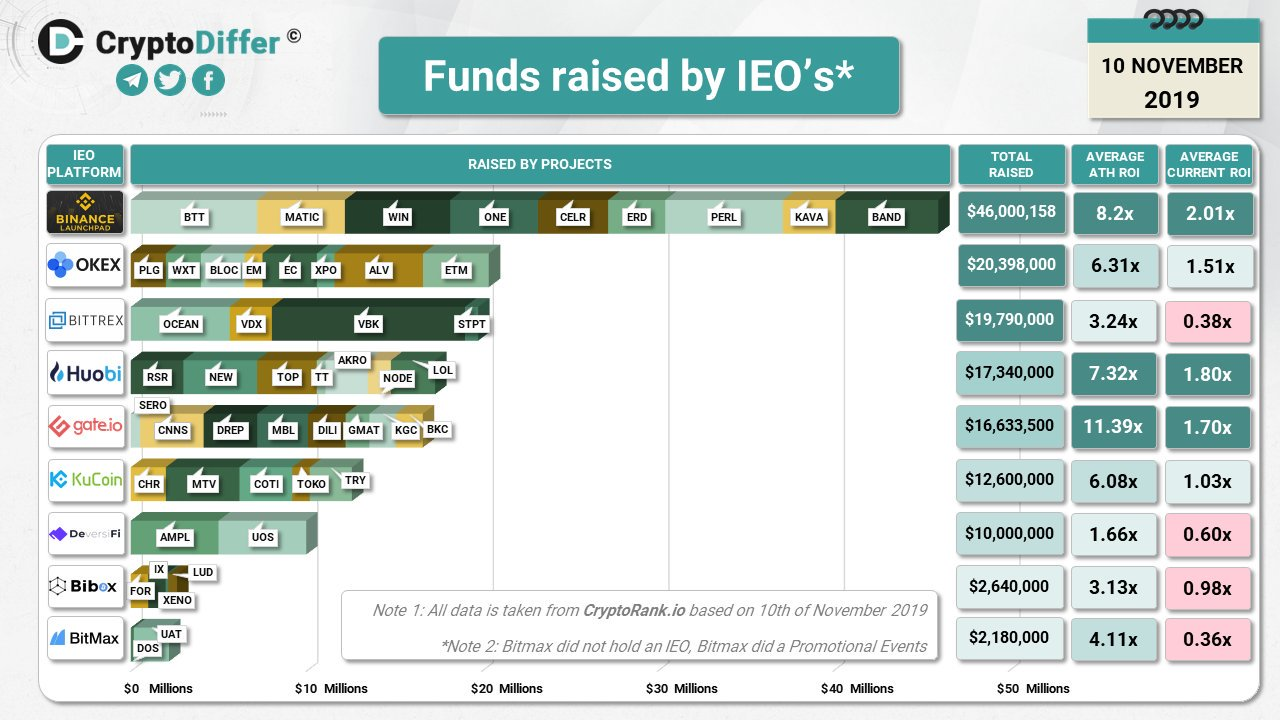
\includegraphics[width=10.5cm]{../pics/cryptocurrency/IEO_raised-20191110}
	\end{figure}
}

\frame{
% 
	\frametitle{Funding by Industry}
	\begin{figure}
		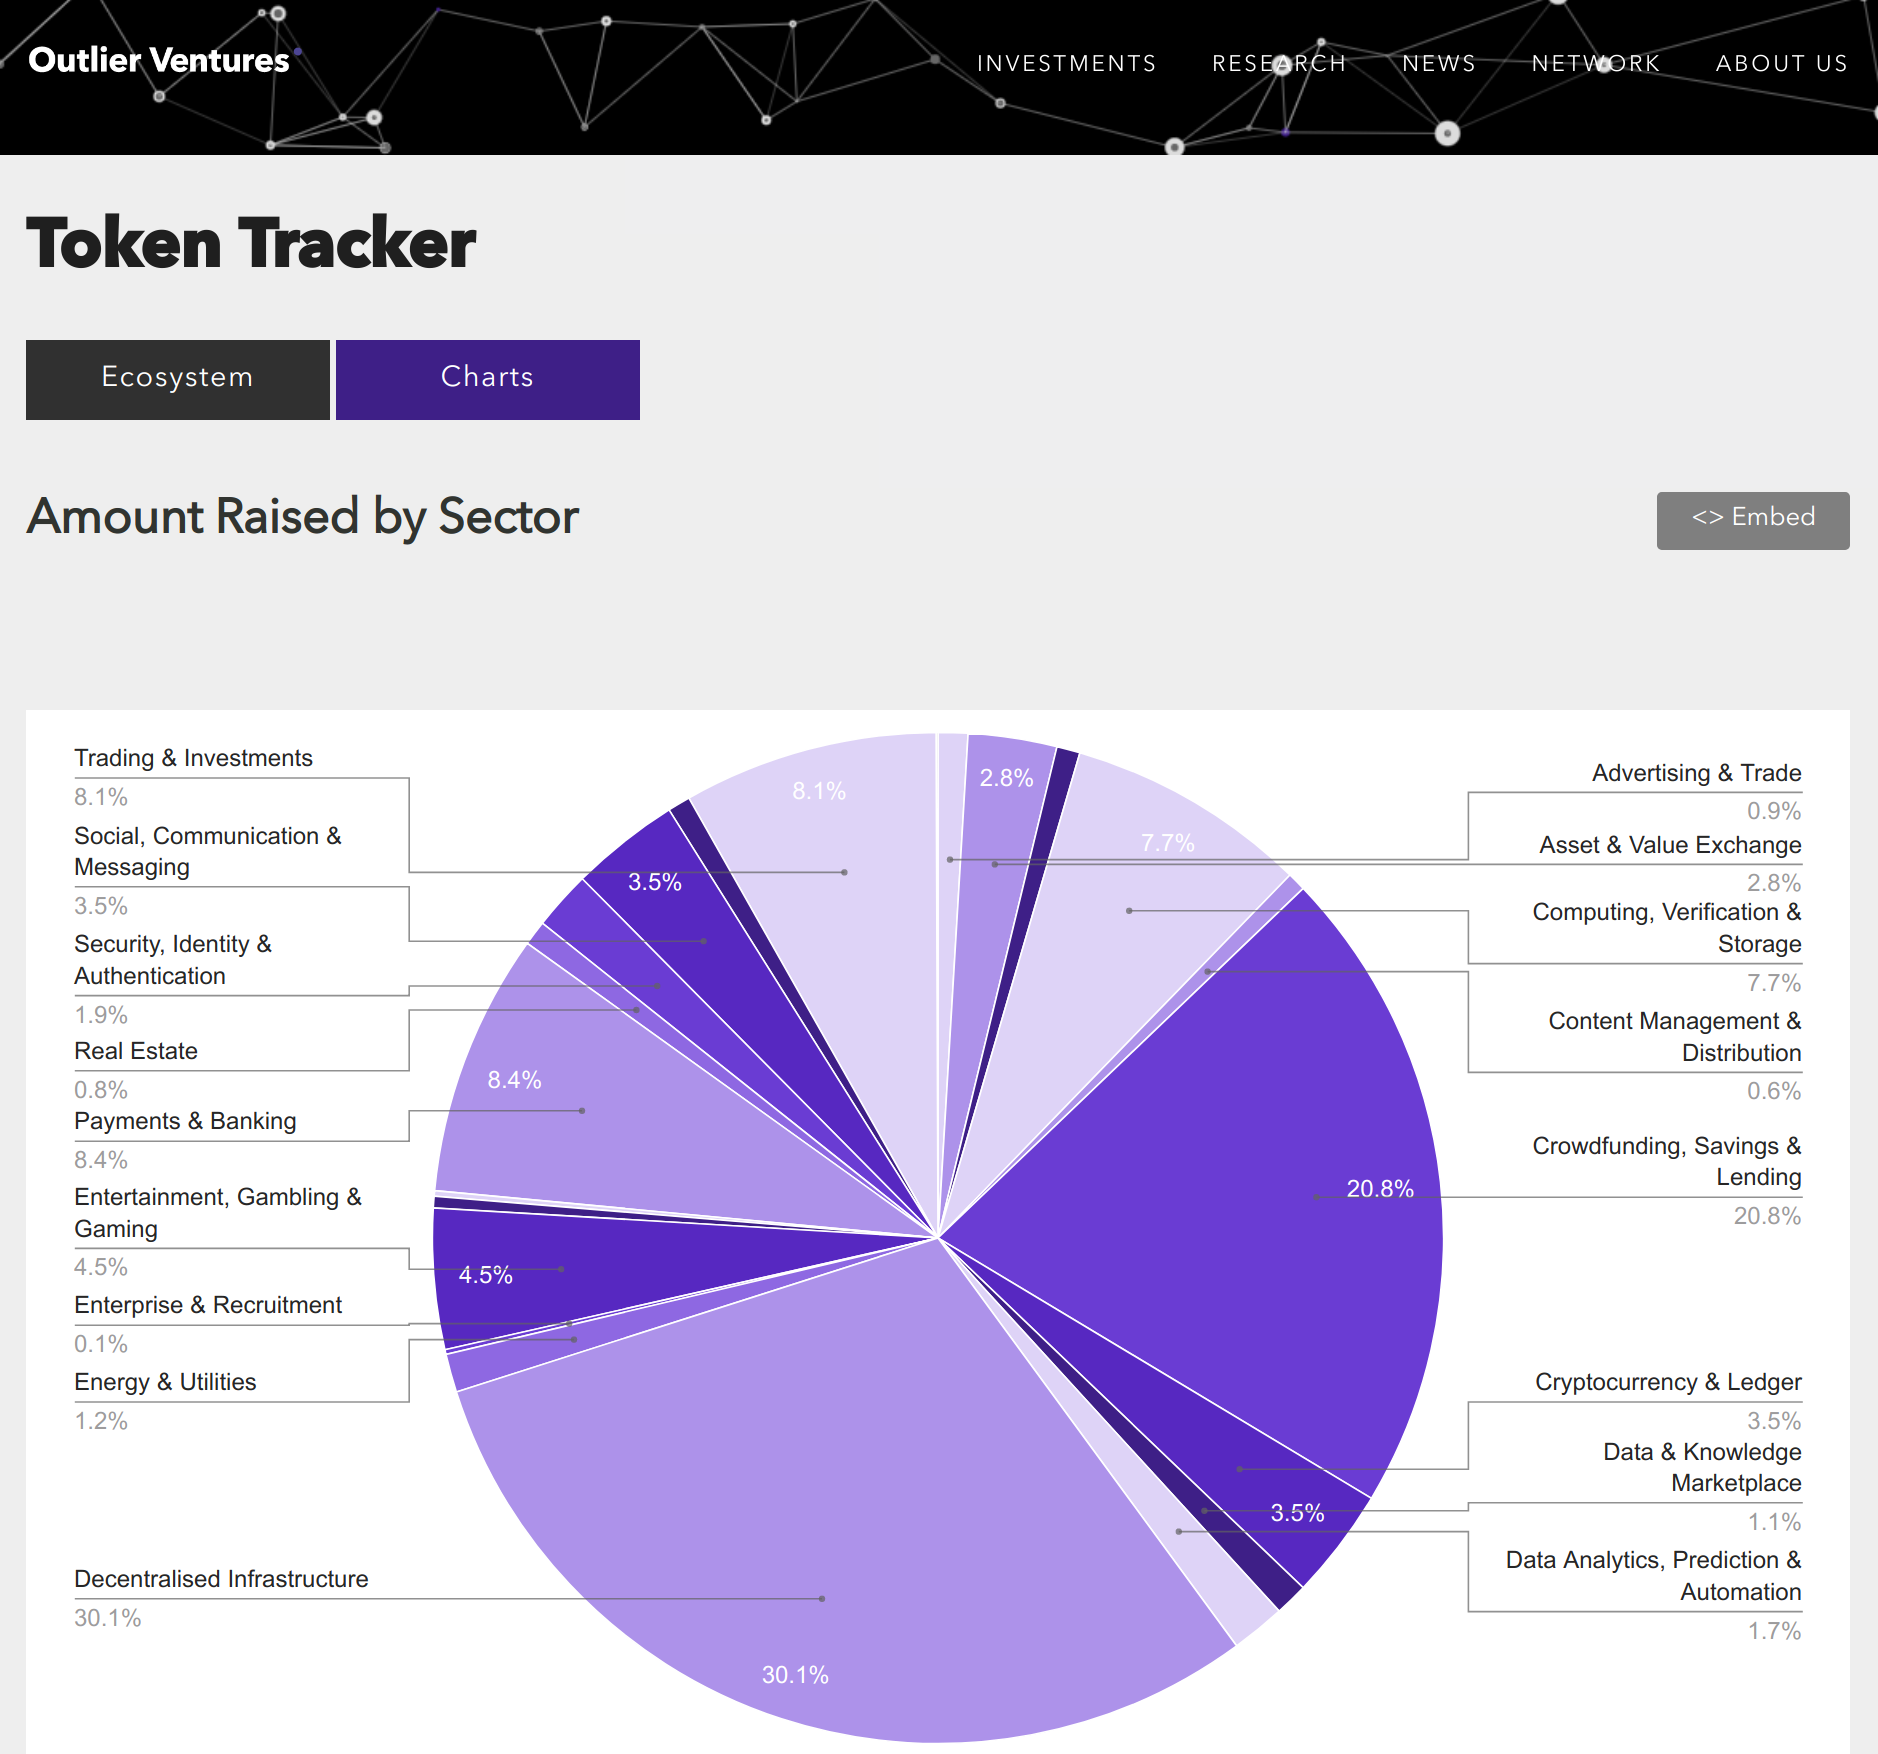
\includegraphics[height=6.5cm]{../pics/cryptocurrency/outlier-token-tracker}
	\end{figure}
}

\frame{
    \frametitle{References}
    \url{https://icobench.com} \\
    \url{https://topicolist.com} \\
    \url{https://icostats.com}  \\
}


% ======================================================================================================
%                         Elements of a good white paper 
% ======================================================================================================
% - framework to use for students
\section{What makes a good white paper}


\frame{
    \frametitle{Who buys into ICOs?}

    \center\Huge  Elements of a white paper
}

\subsection{Criteria}

\frame{ 
	\frametitle{General considerations}
    \begin{alertblock}{Be careful with your money}
    Any investment requires due diligence. Ask yourself what the investor gets for his/her money?
    \end{alertblock}

    \begin{alertblock}{Guarantees}
    How confident are you the team will complete its end of the bargain? What are the available recourse when they do not?
    \end{alertblock}

    \begin{alertblock}{Compliance}
    Is this legal? What are the risks and the administrative burden on the investor side?
    % example: illegal trafficking of substances, duty to report to CRA and other regulators
    \end{alertblock}

}


\frame{ 
	\frametitle{Team}
    \begin{itemize}
        \item Do these people exist?
        \item Do their roles and credentials match the domain of expertise?
        \item Did they agree to be featured? 
        \item How much are they involved in the project? (100\% time -- 0.001\% time?)
        \item Are they credible? Can they pull it off?
        \item Which company is backing this project (if any)?
    \end{itemize}
}

\frame{ 
	\frametitle{Project}
    \begin{itemize}
        \item Does it have any kind of business or social value? 
        \item What is the business model (including token economics)?
        \item Is it achievable? (There should be a sensical roadmap)
        \item How much research and development has already been done so far?
        \item How many users are currently using the system (if any)? (is there a MVP?)
    \end{itemize}
}

\frame{ 
	\frametitle{Technology}
    \begin{itemize}
        \item Why do we need Blockchain for that?
        \item Is Blockchain (and other) technology used apropriately?
% a study from UBC shows that half of the projects don't need a blockchain https://editorialexpress.com/cgi-bin/conference/download.cgi?db_name=CICF2019&paper_id=1043
        \item What is the underlying Blockchain platform? (e.g. Ethereum, Waves)
        \item How are the engineering constraints addressed? (e.g. throughput in tps, scalability, saturation, cost of transactions, interoperability)
        \item How maintainable and sustainable the solution is?
        \item What is the approach to ensure an acceptable level of security?
    \end{itemize}
}

\frame{ 
	\frametitle{Governance and Use of the proceeds}
    \begin{itemize}
        \item What does the team plan to do with the funds?
        \item What is the governance model?
        \item What's in there for the investor?
        \item Is the financial model realistic?
        \item Are legal and compliance risks thorougly assessed and discussed?
    \end{itemize}
}

\frame{ 
	\frametitle{ICO process}
    \begin{itemize}
        \item How is the token issued? (e.g. through an exchange)
        \item Are all investors treated fairly? (e.g. similar value/risk ratio, unreasonable pre-sale discounts to a certain class of investors)
        \item Do the founders have an unfair advantage? (e.g. control)
        \item Is the ICO backed to some level by regulators? (e.g. the OSC in Ontario can issue exemption letters, SEC in the US)
        \item What does the crypto-community say? (e.g. coverage in journals, podcasts, Youtube, Reddit, etc)
    \end{itemize}
}


\frame{
	\frametitle{Putting it all together: a framework to assess white papers}
    \framesubtitle{\href{https://docs.google.com/spreadsheets/d/1qME74KlDxLJk0vcbHq5ZBQp3b9B79S_WejP9izOQWHo/edit?usp=sharing}{Template on Google Drive}}
	\begin{figure}
		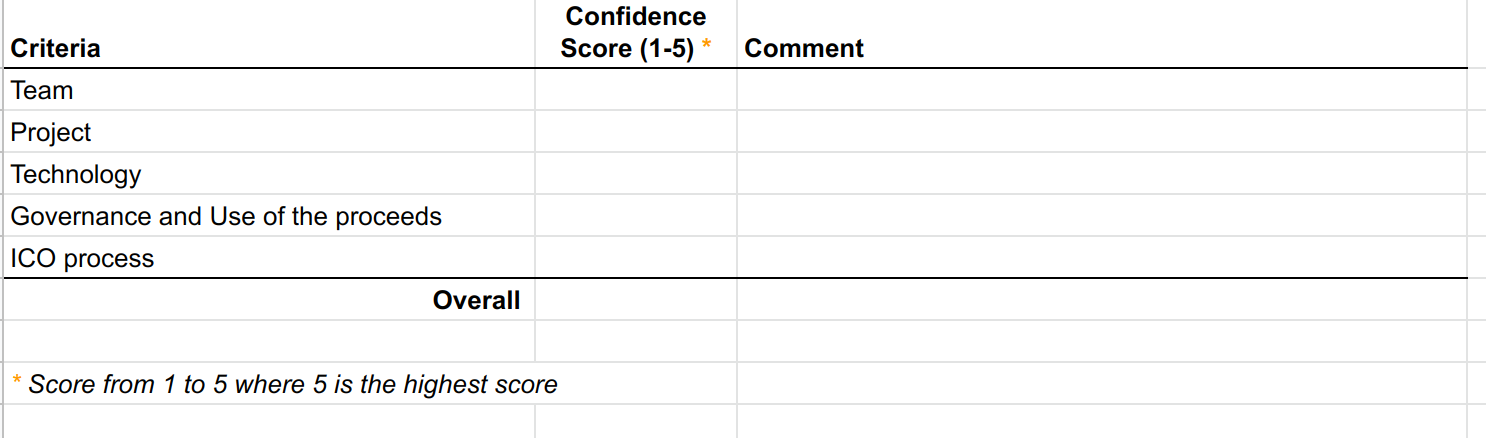
\includegraphics[width=11.5cm]{../pics/cryptocurrency/ico-analysis-fwk}
	\end{figure}
}



